\documentclass[ignorenonframetext,12pt]{beamer}
\usepackage[ngerman]{babel}
\usepackage[T1]{fontenc}
\usepackage[utf8]{inputenc}

%%%%%%%%%%%%%%%%%%%%%%%%%%%%%%%%%%%%%%%%%%%%%%%%%%%%%%%%%%%%%%%%%%%%%%%%%%%%%%%%
%%%%%%%%%%%%%%%%%%%%%%%%%%%%%%%%%%%%%%%%%%%%%%%%%%%%%%%%%%%%%%%%%%%%%%%%%%%%%%%%
%
% A general frame for lecture slides and lecture notes in one file
% using LaTeX beamer
%
%%%%%%%%%%%%%%%%%%%%%%%%%%%%%%%%%%%%%%%%%%%%%%%%%%%%%%%%%%%%%%%%%%%%%%%%%%%%%%%%
%%%%%%%%%%%%%%%%%%%%%%%%%%%%%%%%%%%%%%%%%%%%%%%%%%%%%%%%%%%%%%%%%%%%%%%%%%%%%%%%

% only for the article version
\mode<article>
{
  \usepackage[automark,komastyle]{scrpage2}
  \usepackage{amsfonts}
  \usepackage{amscd}
  %\usepackage[headings]{fullpage}
%  \setlength{\parindent}{0pt}
%  \setlength{\parskip}{1.25ex plus 0.5ex minus 0.2ex}
}

% only presentation
\mode<presentation>
{
\usetheme{default}
\usepackage{multimedia}
\setbeamercovered{transparent}
\usefonttheme{structurebold}
\setbeamertemplate{theorems}[numbered]
\usepackage{amscd}
}

%% support '.' in pdf file names
\usepackage{grffile}

% all after
\usepackage{tikz}
\usepackage{eurosym}
\usepackage{graphicx}
%\usepackage{psfrag}
\usepackage{listings}
\lstset{language=C++, basicstyle=\ttfamily,
  keywordstyle=\color{red}\bfseries, tabsize=4, stringstyle=\ttfamily,
  commentstyle=\itshape, extendedchars=true, inputencoding=utf8, texcl=true, escapeinside={/*@}{@*/}}
\usepackage{curves}
%\usepackage{epic}
\usepackage{calc}
\usepackage{picinpar}
%\usepackage{fancybox}
%\usepackage{xspace}
\usepackage{enumerate}
\usepackage{algorithmic}
\usepackage{algorithm}
\usepackage{bm}
\usepackage[german]{varioref}
\usepackage{bibgerm}
%\usepackage{multibib}
\usepackage{nicefrac}
\usepackage{cite}

\mode<article> {
%  \usepackage[dvips,a4paper]{hyperref}
  \usepackage[%
  pagebackref=false, % bibliography -> text
  linktocpage=true, % toc etc: make page number active (not name)
  plainpages=false, % distinguish roman and arabic pagenumbers
  bookmarksopen=true,%
  bookmarksnumbered=true,%
  pdfauthor={Peter Bastian},%
  pdftitle={Heidelberger Numerikbibliothek für die Lehre},%
  pdfsubject={},%
  pdfkeywords={},%
]{hyperref}        % clickabe references
  \usepackage{multimedia}
  \usepackage{cite}
  \setkomafont{pagenumber}{\normalfont\scshape}
  \setkomafont{pageheadfoot}{\normalfont\scshape}
}
%\usepackage{breakurl}

%\newcites{num}{Lehrbücher Numerik}
%\newcites{cpp}{Lehrbücher C++}

%The theorems
\mode<presentation>
{
\theoremstyle{definition}
}
\mode<article>
{
\theoremstyle{definition}
}

\newtheorem{Def}{Definition}[section]
\newtheorem{Bsp}[Def]{Beispiel}
\newtheorem{Bem}[Def]{Bemerkung}
\newtheorem{Lem}[Def]{Lemma}
\newtheorem{Rgl}[Def]{Regel}
\newtheorem{Sat}[Def]{Satz}
\newtheorem{HSatz}[Def]{Hilfssatz}
\newtheorem{Kor}[Def]{Korollar}
\newtheorem{Folg}[Def]{Folgerung}
\newtheorem{Beob}[Def]{Beobachtung}
\newtheorem{wissen}[Def]{Wissen}
\newtheorem*{geschichte}{Geschichte}


%\newtheorem{Def}{Definition}[section]
%\newtheorem{Exm}[Def]{Example}
%\newtheorem{Lem}[Def]{Lemma}
%\newtheorem{Rem}[Def]{Remark}
%\newtheorem{Rul}[Def]{Rule}
%\newtheorem{Thm}[Def]{Theorem}
%\newtheorem{Cor}[Def]{Corollary}
%\newtheorem{Obs}[Def]{Observation}
%\newtheorem{Ass}[Def]{Assumption}
%\newtheorem{Pro}[Def]{Property}
%\newtheorem{Alg}[Def]{Algorithm}
%\newtheorem{Prp}[Def]{Proposition}
%\newtheorem{Lst}[Def]{Listing}

% Delete this, if you do not want the table of contents to pop up at
% the beginning of each subsection:
%\AtBeginSection[]
%{
%  \begin{frame}<beamer>
%    \frametitle{Contents}
%\tableofcontents[currentsection,sectionstyle=show/hide,subsectionstyle=show/show/hide]
%    \tableofcontents[currentsection]
%  \end{frame}
%}

% Title definition
\mode<presentation>
{
  \title{Ein kleiner Programmierkurs}
  \author{Peter Bastian}
  \institute[IWR]
  {
    Universität Heidelberg\\
    Interdisziplinäres Zentrum für Wissenschaftliches Rechnen\\
    Im Neuenheimer Feld 205, D-69120 Heidelberg\\
	email: \url{Peter.Bastian@iwr.uni-heidelberg.de}
  }
  \date{\today}
  %\logo{\includegraphics[width=9mm]{./EPS/iwrlogo-klein}}
}
\mode<article>
{
  \title{Heidelberger Numerikbibliothek \\ für die Lehre}
  \author{\textsc{Peter Bastian}\\
    Universität Heidelberg\\
    Interdisziplinäres Zentrum für Wissenschaftliches Rechnen\\
    Im Neuenheimer Feld 205, D-69120 Heidelberg\\
	email: \url{Peter.Bastian@iwr.uni-heidelberg.de}
  }
  \date{\today}
}

% logo nach oben
\mode<presentation>
{
% No navigation symbols and no lower logo
\setbeamertemplate{sidebar right}{}

% logo
\newsavebox{\logobox}
\sbox{\logobox}{%
    \hskip\paperwidth%
    \rlap{%
      % putting the logo should not change the vertical possition
      \vbox to 0pt{%
        \vskip-\paperheight%
        \vskip0.35cm%
        \llap{\insertlogo\hskip0.1cm}%
        % avoid overfull \vbox messages
        \vss%
      }%
    }%
}

\addtobeamertemplate{footline}{}{%
    \usebox{\logobox}%
}
}

% number equations within sections in article mode
%\numberwithin{equation}{section}

% math symbols
\newcommand{\diffd}{\,d}

%%%%%%%%%%%%%%%%%%%%%%%%%%%%%%%%%%%%%%%%%%%%%%%%%%%%%%%%%%%%%%%%%%%%%%%%%%%%%%%%
%%%%%%%%%%%%%%%%%%%%%%%%%%%%%%%%%%%%%%%%%%%%%%%%%%%%%%%%%%%%%%%%%%%%%%%%%%%%%%%%
%
% now comes the individual stuff lecture by lecture
%
%%%%%%%%%%%%%%%%%%%%%%%%%%%%%%%%%%%%%%%%%%%%%%%%%%%%%%%%%%%%%%%%%%%%%%%%%%%%%%%%
%%%%%%%%%%%%%%%%%%%%%%%%%%%%%%%%%%%%%%%%%%%%%%%%%%%%%%%%%%%%%%%%%%%%%%%%%%%%%%%%
\mode<article>
{
\pagestyle{scrheadings}
}

\begin{document}
\nocite{*}
\mode<presentation>
{
  \begin{frame}
    \titlepage
  \end{frame}
}
\mode<article>
{
\maketitle
}

\begin{abstract}
Die Heidelberger Numerikbibliothek wurde begleitend zu den Vorlesungen
\textit{Einführung in die Numerik} und \textit{Numerik} in der Programmiersprache C++
entwickelt und stellt
einfach zu benutzende Klassen für grundlegende Aufgaben in der Numerik bis hin zur Lösung
von gewöhnlichen Differentialgleichungen zur Verfügung. In fast allen Klassen ist der
benutzte Zahlentyp parametrisierbar so dass auch hochpräzise Rechnungen durchgeführt werden können.
\end{abstract}

%\mode<presentation>{
%\begin{frame}<presentation>
%\frametitle{Outline}
%\tableofcontents[section,sectionstyle=show/show,subsectionstyle=hide/hide/hide]
%\end{frame}
%}


%%%%%%%%%%%%%%%%%%%%%%%%%%%%%%%%%%%%%%%%%%%%%%%%%%%%%%%%%%%%%%%
% Die Kapitel
%%%%%%%%%%%%%%%%%%%%%%%%%%%%%%%%%%%%%%%%%%%%%%%%%%%%%%%%%%%%%%%

\section{Ein kleiner Programmierkurs}

\subsection{Hallo Welt}

\begin{frame}[fragile]
\frametitle{Programmierumgebung}
\begin{itemize}
\item Wir benutzen die Programmiersprache C++.
\item Wir behandeln nur die Programmierung unter LINUX mit den GNU
  compilern.
\item Windows: On your own.
\item Wir setzen Grundfertigkeit im Umgang mit LINUX-Rechnern voraus:
\begin{itemize}
\item Shell, Kommandozeile, Starten von Programmen.
\item Dateien, Navigieren im Dateisystem.
\item Erstellen von Textdatein mit einem Editor ihrer Wahl.
\end{itemize}
\item Idee des Kurses: \glqq{}Lernen an Beispielen\grqq{}, keine
  rigorose Darstellung.
\item Blutige Anfänger sollten zusätzlich ein Buch lesen.
\end{itemize}
\end{frame}

\begin{frame}[fragile]
\frametitle{Workflow}
C++ ist eine \glqq{}kompilierte\grqq{} Sprache. Um ein Programm zur
Ausführung zu bringen sind folgende Schritte notwendig:
\begin{enumerate}
\item Erstelle/Ändere den Programmtext mit einem \textbf{Editor}.
\item Übersetze den Programmtext mit dem \textbf{C++-Übersetzer}
  (auch C++-Compiler) in ein Maschinenprogramm.
\item Führe das Programm aus. Das Programm gibt sein Ergebnis auf dem
  Bildschirm oder in eine Datei aus.
\item Interpretiere Ergebnisse. Dazu benutzen wir weitere Programme
  wie \textbf{gnuplot} oder \textbf{grep}.
\item Falls Ergebnis nicht korrekt, gehe nach 1!
\end{enumerate}
\end{frame}

\begin{frame}[fragile]
\frametitle{HDNUM}
\begin{itemize}
\item C++ kennt keine Matrizen, Vektoren, Polynome, \ldots
\item Wir haben C++ erweitert um die \textbf{Heidelberg Educational
  Numerics Library}, kurz \textbf{HDNum}.
\item Alle in der Vorlesung behandelten Beispiele sind dort
  enthalten.
\item Dieser Programmierkurs ist auch Teil von HDNUM
\end{itemize}
\end{frame}

\begin{frame}
\frametitle{Herunterladen von HDNUM }
\begin{enumerate}
\item Einloggen
\item Herunterladen von HDNUM\\
\texttt{\tiny git clone https://parcomp-git.iwr.uni-heidelberg.de/Teaching/hdnum.git}
\item Wechsle in das Verzeichnis \\ \lstinline{$ cd hdnum/examples/progkurs} %$
\item Anzeigen der Dateien mittels\\ \lstinline{$ ls} %$
\end{enumerate}
\end{frame}

\begin{frame}
\frametitle{Wichtige UNIX-Befehle}
\begin{itemize}
\item \lstinline{ls --color -F} - Zeige Inhalt des aktuellen Verzeichnisses
\item \lstinline{cd} - Wechsle ins Home-Verzeichnis
\item \lstinline{cd <verzeichnis>} - Wechsle in das angegebene
  Verzeichnis (im aktuellen Verzeichnis)
\item \lstinline{cd ..} - Gehe aus aktuellem Verzeichnis heraus
\item \lstinline{mkdir < verzeichnis>} - Erstelle neues Verzeichnis
\item \lstinline{cp <datei1> <datei2>} - Kopiere datei1 auf datei2
  (datei2 kann durch Verzeichnis ersetzt werden)
\item \lstinline{mv <datei1> <datei2>} - Benenne datei1 in datei2 um
  (datei2 kann durch Verzeichnis ersetzt werden, dann wird datei1
  dorthin verschoben)
\item \lstinline{rm <datei>} - Lösche datei
\item \lstinline{rm -rf <verzeichnis>} - Lösche Verzeichnis mit allem darin
\end{itemize}
\end{frame}

\begin{frame}[fragile]
\frametitle{Hallo Welt !}
Öffne die Datei \lstinline{hallohdnum.cc} mit einem Editor:
\\ \lstinline{$ gedit hallohdnum.cc} %$
\lstinputlisting[basicstyle=\ttfamily\scriptsize,numbers=left,
numberstyle=\tiny, numbersep=5pt]{../examples/progkurs/hallohdnum.cc}
\begin{itemize}
\item \lstinline{iostream} ist eine sog. \glqq{}Headerdatei\grqq{}
\item \lstinline!#include! erweitert die \glqq{}Basissprache\grqq{}.
\item \lstinline!int main ()! braucht man immer: \glqq{}Hier geht's los\grqq{}.
\item \lstinline!{ ... }! klammert Folge von Anweisungen.
\item Anweisungen werden durch Semikolon abgeschlossen.
\end{itemize}
\end{frame}

\begin{frame}[fragile]
\frametitle{Hallo Welt laufen lassen}
\begin{itemize}
\item Gebe folgende Befehle ein:
{\small\begin{lstlisting}{}
$ g++ -I../../ -o hallohdnum hallohdnum.cc
$ ./hallohdnum
\end{lstlisting}}
\item Dies sollte dann die folgende Ausgabe liefern:
{\small\begin{lstlisting}{}
Numerik 0 ist ganz leicht!
1+1=2
\end{lstlisting}}
\end{itemize}
\end{frame}

\subsection{Variablen und Typen}

\begin{frame}[fragile]
\frametitle{(Zahl-) Variablen}
\begin{itemize}
\item Aus der Mathematik: \glqq{}$x\in M$\grqq{}. Variable $x$ nimmt einen
  beliebigen Wert aus der Menge $M$ an.
\item Geht in C++ mit: \lstinline{    M x;}
\item \textbf{Variablendefinition}:
\lstinline{x} ist eine Variable vom \textbf{Typ} \lstinline{M}.
\item Mit \textbf{Initialisierung}: \lstinline{    M x(0);}
\item Wert von Variablen der \glqq{}eingebauten\grqq{} Typen ist sonst
  nicht definiert.
\end{itemize}
\lstinputlisting[basicstyle=\ttfamily\scriptsize,numbers=left,
numberstyle=\tiny, numbersep=5pt]{../examples/progkurs/zahlen.cc}
\end{frame}

\begin{frame}[fragile]
\frametitle{Andere Typen}
\begin{itemize}
\item C++ kennt noch viele weitere Typen.
\item Typen können nicht nur Zahlen sondern viele andere Informationen
  repräsentieren.
\item Etwa Zeichenketten: \lstinline{std::string}
\item Oft muss man dazu weitere Headerdateien angeben.
\lstinputlisting[basicstyle=\ttfamily\scriptsize,numbers=left,
numberstyle=\tiny, numbersep=5pt]{../examples/progkurs/string.cc}
\item Jede Variable \textsl{muss} einen Typ haben. Strenge Typbindung.
\end{itemize}
\end{frame}

\begin{frame}[fragile]
\frametitle{Mehr Zahlen}
\lstinputlisting[basicstyle=\ttfamily\scriptsize,numbers=left,
numberstyle=\tiny, numbersep=5pt]{../examples/progkurs/mehrzahlen.cc}
\begin{itemize}
\item GNU Multiprecision Library \url{http://gmplib.org/} erlaubt
  Zahlen mit vielen Stellen (hier 512 Stellen zur Basis 2).
\item übersetzen mit:\\
{\scriptsize\lstinline{$ g++ -I../../ -o mehrzahlen mehrzahlen.cc -lgmpxx -lgmp}} %$
\item Komplexe Zahlen sind Paare von Zahlen.
\item \lstinline{complex<>} ist ein Template: Baue komplexe Zahlen aus
  jedem anderen Zahlentyp auf (später mehr!).
\end{itemize}
\end{frame}

\begin{frame}[fragile]
\frametitle{Mehr Ein- und Ausgabe}
\lstinputlisting[basicstyle=\ttfamily\scriptsize,numbers=left,
numberstyle=\tiny, numbersep=5pt]{../examples/progkurs/eingabe.cc}
\begin{itemize}
\item Eingabe geht mit \lstinline{std::cin >> x;}
\item Standardmäßig werden nur 6 Nachkommastellen ausgegeben. Das
  ändert man mit \lstinline{std::setprecision}.
\item Dazu muss man die Headerdatei \lstinline{iomanip} einbinden.
\item Die Wurzel berechnet die Funktion \lstinline{sqrt}.
\end{itemize}
\end{frame}

\begin{frame}[fragile]
\frametitle{Zuweisung}
\begin{itemize}
\item Den Wert von Variablen kann man ändern. Sonst wäre es langweilig
  :-)
\item Dies geht mittels Zuweisung:
{\scriptsize\begin{lstlisting}{}
double x(3.14); // Variablendefinition mit Initialisierung
double y;       // uninitialisierte Variable
y = x;          // Weise y den Wert von x zu
x = 2.71;       // Weise x den Wert 2.71, y unverändert
y = (y*3)+4;    // Werte Ausdruck rechts von = aus
                // und weise das Resultat y zu!
\end{lstlisting}}
\end{itemize}
\end{frame}

\begin{frame}[fragile]
\frametitle{Blöcke}
\begin{itemize}
\item Block: Sequenz von Variablendefinitionen und Zuweisungen in
  geschweiften Klammern.
{\scriptsize\begin{lstlisting}{}
{
  double x(3.14);
  double y;
  y = x;
}
\end{lstlisting}}
\item Blöcke können rekursiv geschachtelt werden.
\item Eine Variable ist nur in dem Block \textsl{sichtbar} in dem sie
  definiert ist sowie in allen darin enthaltenen Blöcken:
{\scriptsize\begin{lstlisting}{}
{
  double x(3.14);
  {
    double y;
    y = x;
  }
  y = (y*3)+4; // geht nicht, y nicht mehr sichtbar.
}
\end{lstlisting}}
\end{itemize}
\end{frame}

\begin{frame}[fragile]
\frametitle{Whitespace}
\begin{itemize}
\item Das Einrücken von Zeilen dient der besseren Lesbarkeit,
  notwendig ist es (fast) nicht.
\item \lstinline{#include}-Direktiven müssen \textsl{immer} einzeln
  auf einer Zeile stehen.
\item Ist das folgende Programm lesbar?
\lstinputlisting[basicstyle=\ttfamily\scriptsize,numbers=left,
numberstyle=\tiny, numbersep=5pt]{../examples/progkurs/whitespace.cc}
\end{itemize}
\end{frame}

\subsection{Entscheidung}

\begin{frame}[fragile]
\frametitle{\lstinline{If}-Anweisung}
\begin{itemize}
\item Aus der Mathematik kennt man eine \glqq{}Zuweisung\grqq{} der
  folgenden Art.

Für $x\in\mathbb{R}$ setze
\begin{equation*}
y = |x| = \left\{\begin{array}{ll}
x & \text{falls $x\geq 0$}\\
-x & sonst
\end{array}\right.
\end{equation*}
\item Dies realisiert man in C++ mit einer \lstinline{If}-Anweisung:
{\scriptsize\begin{lstlisting}{}
double x(3.14), y;
if (x>=0)
{
  y = x;
}
else
{
  y = -x;
}
\end{lstlisting}}
\end{itemize}
\end{frame}

\begin{frame}[fragile]
\frametitle{Varianten der \lstinline{If}-Anweisung}
\begin{itemize}
\item Die geschweiften Klammern kann man weglassen, wenn der Block nur
  eine Anweisung enthält:
{\scriptsize\begin{lstlisting}{}
double x(3.14), y;
if (x>=0) y = x; else y = -x;
\end{lstlisting}}
\item Der \lstinline{else}-Teil ist optional:
{\scriptsize\begin{lstlisting}{}
double x=3.14;
if (x<0)
  std::cout << "x ist negativ!" << std::endl;
\end{lstlisting}}
\item Weitere Vergleichsoperatoren sind \lstinline{< <= == >= > !=}\\
\item Beachte: \lstinline{=} für Zuweisung, aber \lstinline{==} für den
Vergleich zweier Objekte!
\end{itemize}
\end{frame}


\subsection{Wiederholung}

\begin{frame}[fragile]
\frametitle{\lstinline{While}-Schleife}
\begin{itemize}
\item Bisher: Sequentielle Abfolge von Befehlen wie im Programm
  angegeben. Das ist langweilig :-)
\item Eine Möglichkeit zur Wiederholung bietet die
  \lstinline{While}-Schleife:

\lstinline{while (} \textsl{Bedingung} \lstinline{)}

\lstinline!{! \textsl{Schleifenkörper} \lstinline!}!

\item Beispiel:
{\scriptsize\begin{lstlisting}{}
int i=0; while (i<10) { i=i+1; }
\end{lstlisting}}

\item Bedeutung:
\begin{enumerate}
\item Teste Bedingung der \lstinline{While}-Schleife
\item Ist diese \textsl{wahr} dann führe Anweisungen im
  Schleifenkörper aus, sonst gehe zur ersten Anweisung nach dem
  Schleifenkörper.
\item Gehe nach 1.
\end{enumerate}
\item Anweisungen im Schleifenkörper beeinflussen normalerweise den Wahrheitswert der
  Bedingung.
\item Endlosschleife: Wert der Bedingung wird nie \textsl{falsch}.
\end{itemize}
\end{frame}

\begin{frame}[fragile]
\frametitle{Pendel (analytische Lösung; \lstinline{while}-Schleife)}
\begin{itemize}
\item Die Auslenkung des Pendels mit der Näherung
  $\sin(\phi)\approx\phi$ und $\phi(0)=\phi_0$, $\phi'(0)=0$ lautet:
$$ \phi(t) = \phi_0 \cos\left(\sqrt{\frac{g}{l}} t\right) .$$
\item Das folgende Programm gibt diese Lösung zu den Zeiten $t_i=i
  \Delta t$, $0\leq t_i \leq T$, $i\in\mathbb{N}_0$ aus:
\end{itemize}
\end{frame}
\begin{frame}[fragile]
\frametitle<presentation>{Pendel (analytische Lösung, \lstinline{while}-Schleife)}
\lstinputlisting[basicstyle=\ttfamily\scriptsize,numbers=left,
numberstyle=\tiny, numbersep=5pt]{../examples/progkurs/pendelwhile.cc}
\end{frame}

\begin{frame}[fragile]
\frametitle{Wiederholung (for-Schleife)}
\begin{itemize}
\item Möglichkeit der Wiederholung: \lstinline{for}-Schleife:

\lstinline{for (} \textsl{Anfang}; \textsl{Bedingung};
\textsl{Inkrement} \lstinline{)}

\lstinline!{! \textsl{Schleifenkörper} \lstinline!}!
\item Beispiel:
{\scriptsize\begin{lstlisting}{}
for (int i=0; i<=5; i=i+1)
{
  std::cout << "Wert von i ist " << i << std::endl;
}
\end{lstlisting}}
\item Enthält der Block nur eine Anweisung dann kann man die
  geschweiften Klammern weglassen.
\item Die \textsl{Schleifenvariable} ist so nur innerhalb des
  Schleifenkörpers sichtbar.
\item Die \lstinline{for}-Schleife kann auch mittels einer
  \textsl{while}-Schleife realisiert werden.
\end{itemize}
\end{frame}

\begin{frame}[fragile]
\frametitle{Pendel (analytische Lösung, \lstinline{for}-Schleife)}
\lstinputlisting[basicstyle=\ttfamily\scriptsize,numbers=left,
numberstyle=\tiny, numbersep=5pt]{../examples/progkurs/pendel.cc}
\end{frame}

\mode<article> {
  \begin{figure}
    \begin{center}
      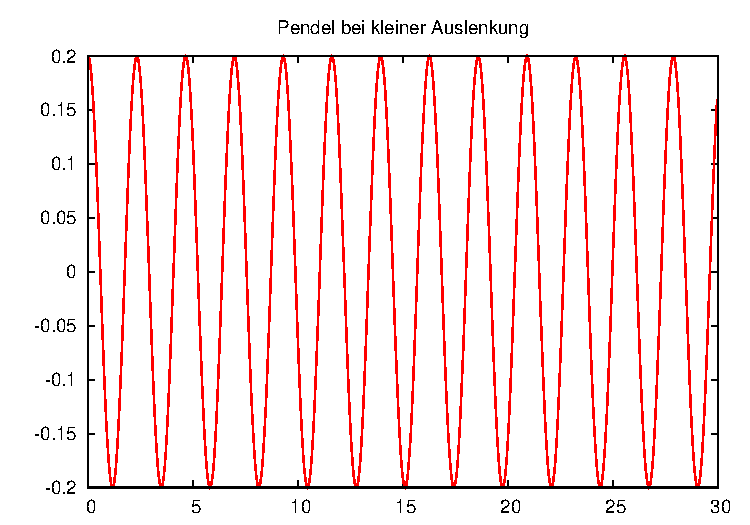
\includegraphics[width=0.8\textwidth]{./pendel}
    \end{center}
    \caption{Das Pendel in Aktion. Gnuplot-Ausgabe des Programmes \lstinline{pendel.cc}.}
    \label{programmierkurs:fig:pendel}
  \end{figure}
}

\begin{frame}
\frametitle{Visualisierung mit \lstinline{Gnuplot}}
\begin{itemize}
\item \lstinline{Gnuplot} erlaubt einfache Visualisierung von Funktionen
  $f:\mathbb{R}\to\mathbb{R}$ und
  $g:\mathbb{R}\times\mathbb{R}\to\mathbb{R}$.
\item Für  $f:\mathbb{R}\to\mathbb{R}$ genügt eine zeilenweise Ausgabe
  von Argument und Funktionswert.
\item Umlenken der Ausgabe eines Programmes in eine Datei:\\
\lstinline{$ ./pendel > pendel.dat}
\item Starte \lstinline{gnuplot}\\
\lstinline{gnuplot> plot "pendel.dat" with lines}
\end{itemize}
\mode<presentation>{
\begin{center}
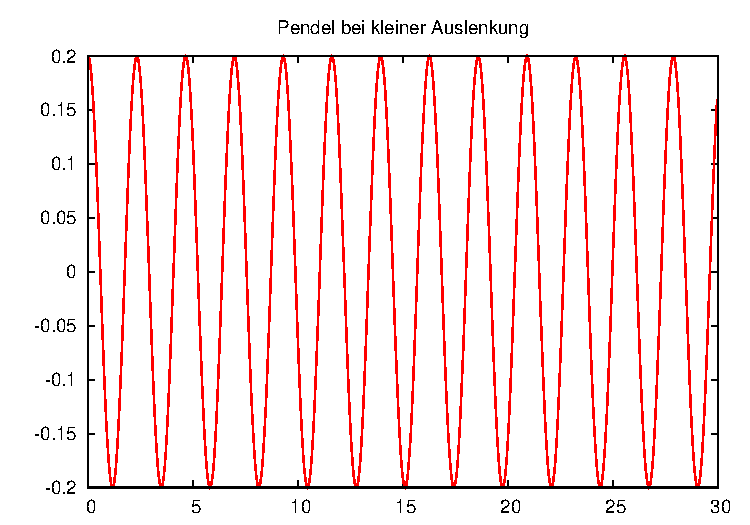
\includegraphics[width=0.4\textwidth]{./pendel}
\end{center}
}
\end{frame}


\begin{frame}[fragile]
\frametitle{Geschachtelte Schleifen}
\begin{itemize}
\item Ein Schleifenkörper kann selbst wieder eine Schleife enthalten,
  man spricht von \textsl{geschachtelten} Schleifen.
\item Beispiel:
{\scriptsize\begin{lstlisting}{}
for (int i=1; i<=10; i=i+1)
  for (int j=1; j<=10; j=j+1)
    if (i==j)
      std::cout << "i gleich j: " << std::endl;
    else
      std::cout << "i ungleich j!" << std::endl;
\end{lstlisting}}
\end{itemize}
\end{frame}

\begin{frame}[fragile]
\frametitle{Numerische Lösung des Pendels}
\begin{itemize}
\item Volles Modell für das Pendel aus der Einführung:
  \begin{gather*}
    \frac{d^2\phi(t)}{d t^2} = - \frac{g}{l} \sin(\phi(t)) \qquad \forall t>0,\\
    \phi(0) = \phi_0, \qquad \frac{d \phi}{d t}(0) = u_0.
  \end{gather*}
\item Umschreiben in System erster Ordnung:
  \begin{align*}
    \frac{d\phi(t)}{d t} &= u(t), & \frac{d^2\phi(t)}{d t^2} &=
    \frac{d u(t)}{d t} = - \frac{g}{l} \sin(\phi(t)).
  \end{align*}
\item Eulerverfahren für $\phi^n = \phi(n\Delta t)$, $u^n = u(n\Delta t)$:
  \begin{align*}
    \phi^{n+1} &= \phi^n + \Delta t \, u^n & \phi^0 &= \phi_0\\
    u^{n+1} &= u^n -\Delta t \, (g/l) \, \sin(\phi^n) & u^0 &= u_0
  \end{align*}
\end{itemize}
\end{frame}

\begin{frame}[fragile]
\frametitle{Pendel (expliziter Euler)}
\lstinputlisting[basicstyle=\ttfamily\scriptsize,numbers=left,
numberstyle=\tiny, numbersep=5pt]{../examples/progkurs/pendelnumerisch.cc}
\end{frame}

\subsection{Funktionen}

\begin{frame}[fragile]
\frametitle{Funktionsaufruf und Funktionsdefinition}
\begin{itemize}
\item In der Mathematik gibt es das Konzept der \textsl{Funktion}.
\item In C++ auch.
\item Sei $f : \mathbb{R} \to \mathbb{R}$, z.B. $f(x) = x^2$.
\item Wir unterscheiden den \textsl{Funktionsaufruf}
{\scriptsize\begin{lstlisting}{}
double x,y;
y = f(x);
\end{lstlisting}}
\item und die \textsl{Funktionsdefinition}. Diese sieht so aus:

\medskip
\textsl{Ergebnistyp} \textsl{Funktionsname} \lstinline{(} \textsl{Argumente} \lstinline{)}

\lstinline!{! \textsl{Funktionsrumpf} \lstinline!}!

\medskip
\item Beispiel:
{\scriptsize\begin{lstlisting}{}
double f (double x)
{
  return x*x;
}
\end{lstlisting}}
\end{itemize}
\end{frame}

\begin{frame}[fragile]
\frametitle{Komplettbeispiel zur Funktion}
\lstinputlisting[basicstyle=\ttfamily\scriptsize,numbers=left,
numberstyle=\tiny, numbersep=5pt]{../examples/progkurs/funktion.cc}
\begin{itemize}
\item Funktionsdefinition muss vor Funktionsaufruf stehen.
\item Formales Argument in der Funktionsdefinition entspricht einer Variablendefinition.
\item Beim Funktionsaufruf wird das Argument (hier) \textsl{kopiert}.
\item \lstinline{main} ist auch nur eine Funktion.
\end{itemize}
\end{frame}

\begin{frame}[fragile]
\frametitle{Weiteres zum Verständnis der Funktion}
\begin{itemize}
\item Der Name des formalen Arguments in der Funktionsdefinition
  ändert nichts an der Semantik der Funktion (Sofern es überall
  geändert wird):

{\scriptsize\begin{lstlisting}{}
double f (double y)
{
  return y*y;
}
\end{lstlisting}}

\item Das Argument wird hier kopiert, d.h.:
{\scriptsize\begin{lstlisting}{}
double f (double y)
{
  y = 3*y*y;
  return y;
}

int main ()
{
  double x(3.0),y;
  y = f(x); // ändert nichts an x !
}
\end{lstlisting}}
\end{itemize}
\end{frame}

\begin{frame}[fragile]
\frametitle{Weiteres zum Verständnis der Funktion}
\begin{itemize}
\item Argumentliste kann leer sein (wie in der Funktion
  \lstinline{main}):
{\scriptsize\begin{lstlisting}{}
double pi ()
{
  return 3.14;
}

y = pi(); // Klammern sind erforderlich!
\end{lstlisting}}

\item Der Rückgabetyp \lstinline{void} bedeutet \glqq{}keine
  Rückgabe\grqq{}

{\scriptsize\begin{lstlisting}{}
void hello ()
{
  std::cout << "hello" << std::endl;
}

hello();
\end{lstlisting}}
\item Mehrere Argument werden durch Kommata getrennt:

{\scriptsize\begin{lstlisting}{}
double g (int i, double x)
{
  return i*x;
}
std::cout << g(2,3.14) << std::endl;
\end{lstlisting}}
\end{itemize}
\end{frame}

\begin{frame}[fragile]
\frametitle{Pendelsimulation als Funktion}
\lstinputlisting[basicstyle=\ttfamily\scriptsize,numbers=left,
numberstyle=\tiny, numbersep=5pt]{../examples/progkurs/pendelmitfunktion.cc}
\end{frame}

\begin{frame}[fragile]
\frametitle{Funktionsschablonen}
\begin{itemize}
\item Oft macht eine Funktion mit Argumenten verschiedenen Typs einen Sinn.
\item \lstinline!double f (double x) {return x*x;}! macht auch mit
  \lstinline{float}, \lstinline{int} oder \lstinline{mpf_class} Sinn.
\item Man könnte die Funktion für jeden Typ definieren. Das ist
  natürlich sehr umständlich. (Es darf mehrere Funktionen gleichen
  Namens geben, sog. \textsl{overloading}).
\item In C++ gibt es mit Funktionsschablonen (engl.: \textsl{function
  templates}) eine Möglichkeit den Typ variabel zu lassen:
{\scriptsize\begin{lstlisting}{}
template<typename T>
T f (T y)
{
  return y*y;
}
\end{lstlisting}}
\item \lstinline{T} steht hier für einen beliebigen Typ.
\end{itemize}
\end{frame}

\begin{frame}[fragile,allowframebreaks]
\frametitle{Pendelsimulation mit Templates}
\lstinputlisting[basicstyle=\ttfamily\scriptsize,numbers=left,
numberstyle=\tiny, numbersep=5pt]{../examples/progkurs/pendelmitfunktionstemplate.cc}
\end{frame}

\begin{frame}[fragile]
\frametitle{Referenzargumente}
\begin{itemize}
\item Das Kopieren der Argumente einer Funktion kann verhindert werden
  indem man das Argument als \textsl{Referenz} definiert:
{\scriptsize\begin{lstlisting}{}
void f (double x, double& y)
{
  y = x*x;
}

double x(3), y;
f(x,y); // y hat nun den Wert 9, x ist unverändert.
\end{lstlisting}}
\item Statt eines Rückgabewertes kann man auch ein (zusätzliches)
  Argument modifizieren.
\item Insbesondere kann man so den Fall mehrerer Rückgabewerte
  realisieren.
\item Referenzargumente bieten sich auch an wenn Argumente \glqq{}sehr
  groß\grqq{} sind und damit das kopieren sehr zeitaufwendig ist.
\item Der aktuelle Parameter im Aufruf \textsl{muss} dann eine Variable sein.
\end{itemize}
\end{frame}

%%%%%%%%%%%%%%%%%%%%%%%%%%%%%%%%%%%%%%%%%%%%%%%%%%%%%%%%%%%%%%%
%%%%%%%%%%%%%%%%%%%%%%%%%%%%%%%%%%%%%%%%%%%%%%%%%%%%%%%%%%%%%%%


% die weiterführende Literatur wollen wir in der Präsentation nie
% zeigen
%\mode<presentation> {
%\begin{frame}<presentation>[allowframebreaks,allowdisplaybreaks]
%  \frametitle{Literatur}
%  \nocite{StoerI}
%  \nocite{Rannacher0}
%  \bibliographystyle{geralpha}
%  \bibliography{lit}
%\end{frame}
%}
%
\end{document}
